\documentclass[a4paper,12pt]{article}

%% Language and font encodings
\usepackage[english]{babel}
\usepackage[utf8x]{inputenc}
\usepackage[T1]{fontenc}
\usepackage{gensymb}

%% Sets page size and margins
\usepackage[a4paper,top=3cm,bottom=2cm,left=3cm,right=3cm,marginparwidth=1.75cm]{geometry}

%% Useful packages
\usepackage{titling}
\usepackage{amsmath}
\usepackage{graphicx}
\usepackage{hyperref}
\usepackage{fancyhdr}
\usepackage{float}
\graphicspath{{graphics/}}
\pagestyle{fancy}


\lhead{Climate App}
\rhead{Instructions}


\title{\vspace{-2.0cm}Climate App instructions\vspace{-2.0cm}}
\date{\today}
\begin{document}

\maketitle
\thispagestyle{fancy}

\section*{What is this ?}

This is a surface application that is used to demonstrate the effects of greenhouse gases on the temperature of a planet. By choosing the value of different parameters shown in the options panel, the user can see a visual representation of the effect on the radiation and temperature. 

\section*{How does it work ?}

This application has a beginner version (figure \ref{fig:ped}) and a advanced version (figure \ref{fig:pro}). The two versions differ in the number of adjustable parameters and, consequently, the complexity of their underlying mathematical relation. You can switch between both versions via the switch located below the title of the page. Switching versions will not reset the parameters. Different components in this application are described below. Some of them appear in both versions under different names, while others are used exclusively in the advanced version.

\begin{figure}[h]
    \centering
    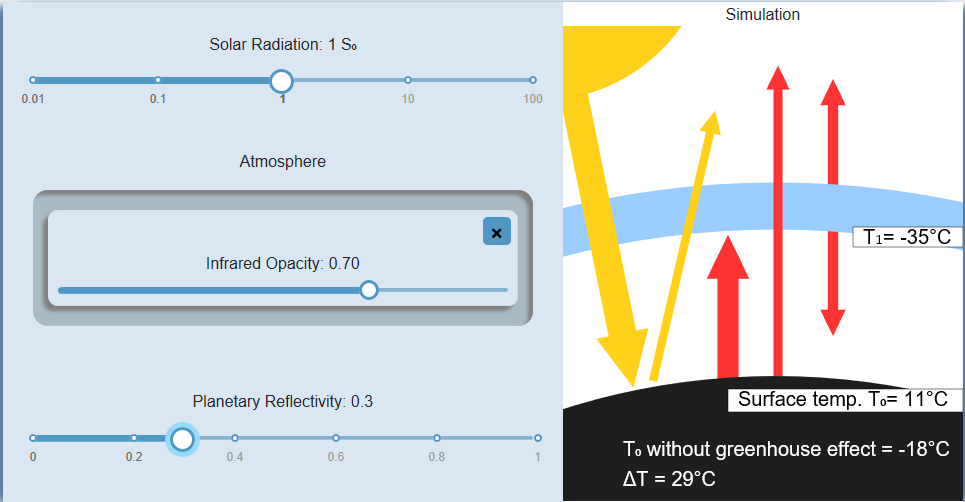
\includegraphics[width=\textwidth]{Ped.PNG}
    \caption{Screenshot of the beginner version.}
    \label{fig:ped}
\end{figure}

\begin{figure}[H]
    \centering
    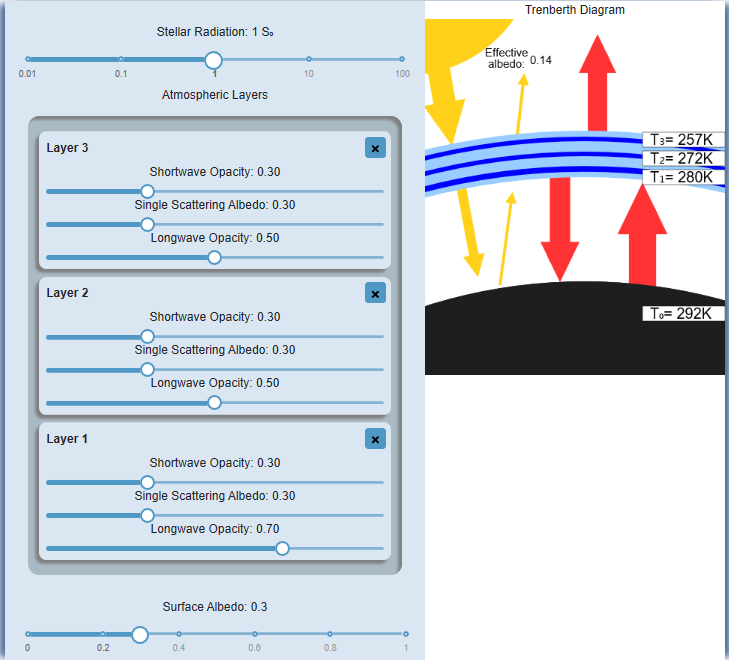
\includegraphics[width=\textwidth]{Pro.PNG}
    \caption{Screenshot of the advanced version.}
    \label{fig:pro}
\end{figure}


\subsection*{Right Panel}

This panel is a visual representation of the planet's climate. The yellow arrows track the shortwave radiation, and the red arrows track the longwave thermal emission. For example, on Earth the incoming sunlight is primarily visible and near infrared, while the outgoing radiation is in the thermal infrared range. By modifying the input variables, it is possible to see the arrows' size varying in real time. The diagram is called a Trenberth Diagram, which uses arrows to visualize global energy flows.

The effect of the solar (or stellar) radiation slider on the total energy flux is not represented on the arrow.\footnote{Since the insolation is a log scale, if we try to visually represent the changes in this parameter in the width of the arrows, all the other modification (e.g. layers' opacity) would have negligible effects and there would be no visible variation.} The widths of arrows therefore represent the fraction of incident flux.

Since there would be a lot of arrows between each layer (see figure \ref{fig:model}), the display of the layers is abstracted in a thick pale blue line. We can still see each layer inside, and their thickness is proportional to their infrared opacity (or longwave emissivity), but the energy exchange between layers of the atmosphere is not shown. The resulting temperatures are shown at the surface and at each layer.

\begin{figure}[H]
  \centering
  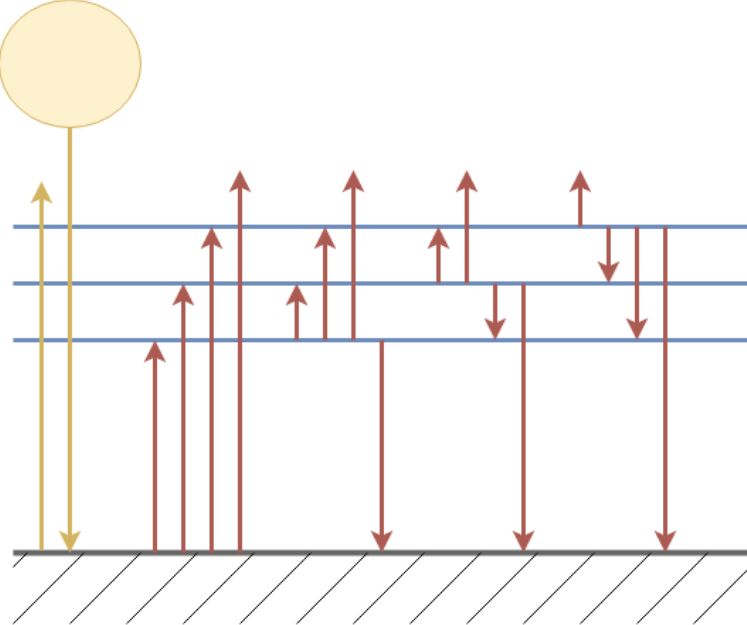
\includegraphics[width=90mm]{Model}
  \caption{Diagram showing how the energy emission and absorption are related at each layer of the atmosphere.}
  \label{fig:model}
\end{figure}

\subsubsection*{Features in Beginner Version}
The two extra temperature displays on the bottom of the simulation emphasize the importance of the greenhouse effect. ``T$_0$ without greenhouse effect'' gives the temperature that the planetary surface would have if it did not have an atmosphere. ``$\Delta $T'' of greenhouse heating gives the difference between the actual surface temperature  and the temperature with infrared opacity set to 0.

\subsubsection*{Feature in Advanced Version}
The effective albedo gives the ratio between the shortwave energy that emerges from the atmosphere and the incoming stellar radiation. It may be different from the user-defined surface albedo, which compares the shortwave radiation absorbed by the surface to the incoming stellar radiation. 

\subsection*{Left Panel}

This panel lets you vary the planetary properties.

\subsubsection*{Solar Radiation or Stellar Radiation}

Also known as ``insolation'', this is the solar or stellar flux at the top of the planetary atmosphere. The solar constant is a quantity measuring the flux density of solar radiation per unit area at a distance of 1 AU (1 astronomical unit i.e. the Earth--Sun distance) from the Sun\footnote{\href{https://en.wikipedia.org/wiki/Solar_constant}{Solar Constant, Wikipedia.}}. The default value of 1 S$_0$ corresponds to approximately 341 W/m$^2$.\footnote{``S$_0$'' corresponds to 1/4 of the solar constant, since the Earth receives solar radiation with a circular cross-section instead of the whole sphere.} For example, a value of 10 on this slider would mean that the planet receives ten times the amount of stellar radiation that we receive on Earth. The slider is a logarithmic scale, which allows for values as high as 100 S$_0$ and as low as 0.01 S$_0$. 


\subsubsection*{Planetary Reflectivity or Surface Albedo}

This value determines how reflective the planetary surface is. A value of 1 would mean that the planet reflects all the incoming radiation. A value of 0 would mean that the planet is very dark and absorbs all the incoming radiation. The default value is the Earth's albedo, approximately 30\%. While moving this slider, you can observe the planet in the simulation canvas change in shade.

\subsubsection*{Atmosphere or Atmospheric Layers}

In this box, you will find settings for the atmosphere. In the beginner version, as shown in figure \ref{fig:ped}, the atmosphere is treated as a single layer to demonstrate the greenhouse effect. You may remove the atmosphere by clicking the $\times$ sign and add it back by clicking on a + box which only appears when your system does not have an atmosphere.

For the advanced version, you may have up to three atmospheric layers, each having different properties. This feature simulates the variation in atmospheric properties within a planetary atmosphere due to different gases. For example, Earth's atmosphere has more water vapor in the lower, warmer layers compared to the higher and colder layers. In this case, lower layers would have higher longwave opacity comparing to higher layers. You can click on the + box to add a new layer, and the $\times$ on a layer to remove it. 

\begin{itemize}
    \item \textbf{Infrared Opacity or Longwave Emissivity}: For each layer in both versions, you can set the value of longwave emissivity, which is its effectiveness in absorbing and emitting energy as thermal radiation. A value of 0 would mean that the layer itself does not emit any thermal radiation; whereas a value of 1 would mean that the layer radiates energy following the Stefan-Boltzmann law (details below).
    
    \item \textbf{Shortwave Opacity}: As shortwave radiation encounters an atmospheric layer, the photons may be transmitted (passing through without interaction), absorbed or scattered by molecules and aerosols in the atmosphere. This slider determines the fraction of interacting (absorbed and scattered) shortwave radiation at the corresponding layer. A value of 1 means that all of the photons interact with this layer, either via absorption or scattering. 
    
    \item \textbf{Single Scattering Albedo}: Single scattering albedo refers to the fraction of interacting photons that are back-scattered rather than absorbed. For example, a value of 0.5 indicates that out of all the photons having interacted with the atmosphere, half of them were scattered instead of being absorbed.
    
\end{itemize}



\section*{Why does it work ?}

There are two concepts that we need to be familiar with to understand how to derive the equations:

\subsection*{Radiative Equilibrium (a.k.a. Energy Balance)}

The total incoming and outgoing energy per unit time (power) must be balanced at each atmospheric layer, including the planetary surface. Imagine a closed parcel of air which receives more energy than it emits. The air parcel therefore warms. Consequently, the parcel's thermal emission increases, which means that it starts radiating more energy outwards and eventually reaches radiative equilibrium, i.e. equal absorbed and emitted power.

In the right panel of this application, the total width of all arrows from the planetary surface should equal the total width of all arrows reaching the surface. The same situation applies for the top of atmosphere.

\subsection*{Stefan-Boltzmann Law\footnote{\href{https://en.wikipedia.org/wiki/Stefan–Boltzmann_law}{Stefan-Boltzmann law, Wikipedia.}}}

The Stefan-Boltzmann law gives a relation between the temperature of an object --- atmospheric layer or planetary surface, in this case --- and the flux it radiates:
\begin{equation*}
    j=\varepsilon \sigma T^4,
\end{equation*}
where $\varepsilon$ is the infrared opacity (or equivalently, the longwave emissivity)\footnote{\href{https://en.wikipedia.org/wiki/Kirchhoff\%27s_law_of_thermal_radiation}{Kirchhoff's law of thermal radiation, Wikipedia.}}, $T$ is the temperature of the object in Kelvin, $j$ is the radiation energy flux and $\sigma$ is the Stefan-Boltzmann constant:
\begin{equation*}
    \sigma=5.6703 \times 10^{-8}\  \text{Watt}/\text{m}^2 \text{K}^4.
\end{equation*}

\subsection*{Deriving the equations}

\subsubsection*{Beginner Version}
In this version we follow the simplest greenhouse model, where the single-layered atmosphere does not interact with the incoming solar radiation. 

\begin{figure}[H]
    \centering
    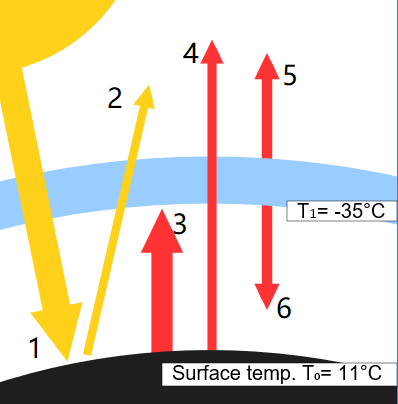
\includegraphics[scale=0.7]{simplemodel.PNG}
    \caption{Simulation used in the beginner version with numbered arrows.}
    \label{fig:simple}
\end{figure}

Figure \ref{fig:simple} gives an illustration of the model that we are analyzing. On the left, we have the incoming solar radiation (1) which is partially absorbed by the surface and partially reflected back into space (2). The surface then heats up and radiates its energy in form of infrared (or longwave) radiation (red arrows). Some of this energy is absorbed by the atmosphere (3), and some of it also makes it into space (4). The atmosphere must radiate away the energy it absorbs from the surface in order to remain in radiative equilibrium. Unlike the surface, the atmosphere radiates both upwards (5) and downwards (6). As shown in figure \ref{fig:simple}, there is a double-sided energy exchange between the planetary surface and the atmosphere. 

Since the temperatures of the surface and the atmosphere are interdependent, we can establish a system of equations to solve for both temperatures. In fact, a more complicated model with three or more layers follows the same principle, where the system of equations may become much more complicated as all layers are interdependent.

The equations for a two-layer model (one atmospheric layer plus the surface) are as following:
\begin{align}
    \sigma T_0^4 & = I(1-\alpha)+\varepsilon_1\sigma T_1^4 \label{eq:t0}\\
    2\varepsilon_1\sigma T_1^4 &= \varepsilon_1\sigma T_0^4,\label{eq:t1} 
\end{align}
where $I$ is the solar (or stellar) radiation, $\alpha$ is the surface albedo and $\varepsilon_1$ is the infrared opacity/longwave emissivity of the atmosphere. We can solve this system of equations analytically as below:

Rearranging the equation \ref{eq:t1} to represent the unknown value $T_1^4$ with known values and the other unknown $T_0^4$:
    $$T_1^4 = \frac{\varepsilon_1\sigma T_0^4}{2\varepsilon_1\sigma}=\frac{T_0^4}{2};$$
    
Plugging the expression of $T_1^4$ into equation \ref{eq:t0}:
    $$\sigma T_0^4  = I(1-\alpha)+\varepsilon_1\sigma \frac{T_0^4}{2};$$
    
Isolating $T_0^4$:
    \begin{align*}
    (\sigma-\frac{\varepsilon_1\sigma}{2})T_0^4&=I(1-\alpha)\\
    T_0^4&=\frac{I(1-\alpha)}{\sigma-\frac{\varepsilon_1\sigma}{2}}\\
    T_0^4&=\frac{2I(1-\alpha)}{\sigma(2-\varepsilon_1)};
    \end{align*}
    
Using the relation between two unknowns to solve for $T_1^4$:
    \begin{align*}
        T_1^4&=\frac{T_0^4}{2}\\
        T_1^4&=\frac{1}{2}\cdot \frac{2I(1-\alpha)}{\sigma(2-\varepsilon_1)}\\
        T_1^4&=\frac{I(1-\alpha)}{\sigma(2-\varepsilon_1)};
    \end{align*}
    
Removing the fourth power to obtain the solutions:
    \begin{align*}
    T_0 &= \Bigg(\frac{2I(1-\alpha)}{\sigma(2-\varepsilon_1)}\Bigg)^{\frac{1}{4}}\\
    T_1 &= \Bigg(\frac{I(1-\alpha)}{\sigma(2-\varepsilon_1)}\Bigg)^{\frac{1}{4}}.
    \end{align*}

As mentioned above, the application's default values are: $I$=341 W/m$^2$, $\alpha=0.3$ and $\varepsilon_1=0.7$. The Stefan-Boltzmann constant $\sigma$ equals to $5.6703 \times 10^{-8}\  \text{Watt/m}^2 \text{K}^4$. By plugging in the numbers into the solutions above, we obtain:
\begin{align*}
    T_0 &= \Bigg(\frac{2\cdot 341(1-0.3)}{5.6703 \times 10^{-8}(2-0.7)}\Bigg)^{\frac{1}{4}}\\
    T_0 &= 283.68 \text{K} \approx 11\degree\text{C}\\
    T_1 &= \Bigg(\frac{341(1-0.3)}{5.6703 \times 10^{-8}(2-0.7)}\Bigg)^{\frac{1}{4}}\\
    T_1 &= 238.55 \text{K} \approx -35\degree\text{C,}\\
\end{align*}
which match the value displayed in figure \ref{fig:ped}.

\subsubsection*{Advanced Version}

Using the same reasoning as the simple greenhouse model, we can derive the system of equations which allow us to solve for the temperatures of planetary surface and three atmospheric layers (see appendix).  However, the model used in advanced version is more complicated. Since we have added two extra parameters related to shortwave radiation, it is now important to analyze the shortwave energy absorbed at each atmospheric layer. Figure \ref{fig:arrow} shows how energy flows within the system. 

\begin{figure}[H]
    \centering
    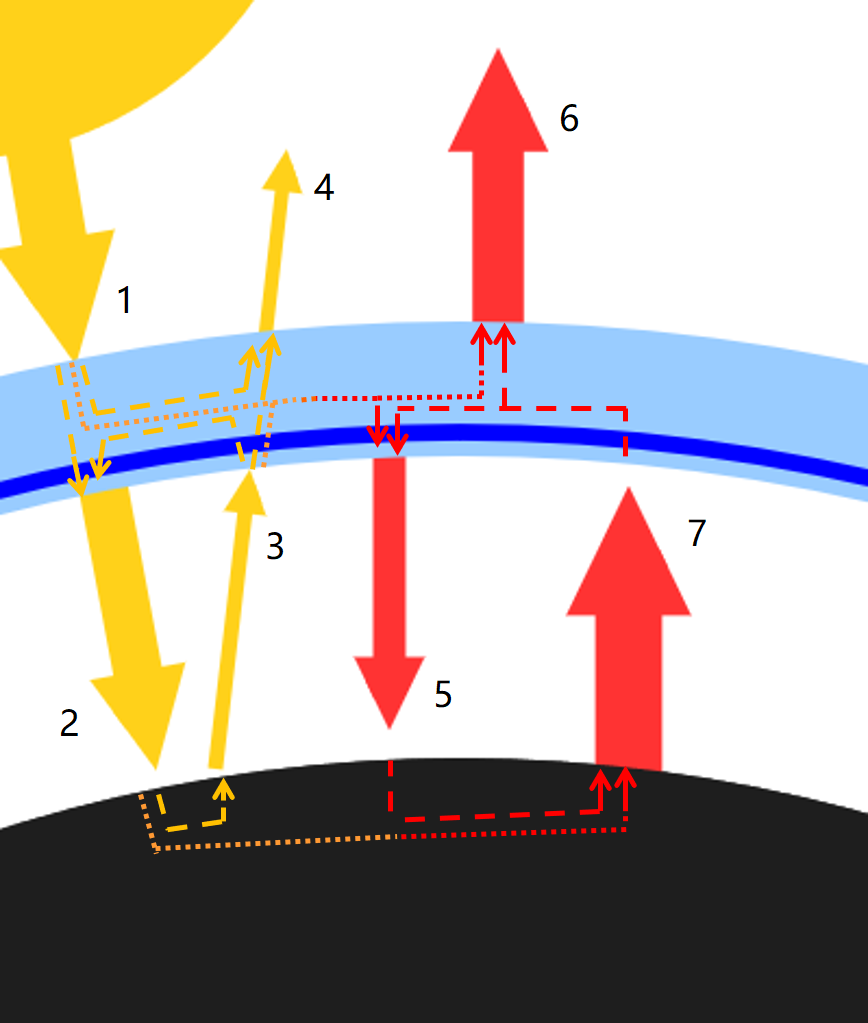
\includegraphics[scale=0.35]{arrow.png}
    \caption{Diagram showing how the various fluxes (arrows in Climate App) are connected to each other for advanced version (beginner version is much simpler).}
    \label{fig:arrow}
\end{figure}

In figure \ref{fig:arrow}, the small arrows with dotted lines indicate detailed energy flows. For example, there are three dotted arrows starting at the end of arrow 1 which represents the stellar radiation reaching top of atmosphere: The left most one joins arrow 2 directly. It represents the fraction of stellar radiation that transmits through the whole atmosphere (including forward-scattering by one or more layers); The middle one, along with a dotted line starting at arrow 3, are connected to arrow 5 and 6. They represent the fraction of stellar radiation that is absorbed by the atmosphere and re-emitted as thermal radiation (arrow 5 and 6); The right most one is connected to arrow 4. It represents the fraction of stellar radiation that is back-scattered by one of the atmospheric layers and exits the atmosphere.

From equation \ref{eq:t0}, we can observe that the term related to shortwave energy, $I(1-\alpha)$, can be viewed as a constant while solving the system of equation, since the variables $T_0,T_1$ are not associated to it. Thus, we can list our equations for the model used in advanced version as following (the Stefan-Boltzmann constant is cancelled on both sides of the equations): 
\begin{align*}
    T_0^4&= \frac{surf}{\sigma} + T_1^4\varepsilon_{lw1} + T_2^4\varepsilon_{lw2}(1-\varepsilon_{lw1}) + T_3^4\varepsilon_{lw3}(1-\varepsilon_{lw2})(1-\varepsilon_{lw1}) \\
 2\varepsilon_{lw1}T_1^4&=\frac{l_1}{\sigma} + T_0^4\varepsilon_{lw1} + T_2^4\varepsilon_{lw1}\varepsilon_{lw2} + T_3^4\varepsilon_{lw1}(1-\varepsilon_{lw2})\varepsilon_{lw3}\\
2\varepsilon_{lw2}T_2^4 &= \frac{l_2}{\sigma} + T_0^4\varepsilon_{lw2}(1-\varepsilon_{lw1}) + T_1^4\varepsilon_{lw1}\varepsilon_{lw2} + T_3^4\varepsilon_{lw2}\varepsilon_{lw3}\\
2\varepsilon_{lw3}T_3^4&= \frac{l_3}{\sigma} + T_0^4\varepsilon_{lw3}(1-\varepsilon_{lw1})(1-\varepsilon_{lw2}) + T_1^4\varepsilon_{lw1}(1-\varepsilon_{lw2})\varepsilon_{lw3}  + T_2^4\varepsilon_{lw2}\varepsilon_{lw3},
\end{align*}
where $\varepsilon_{lwi}$ stands for the longwave emissivity of layer $i$, and "$surf, l_1, l_2, l_3$" represent the shortwave radiation energy absorbed at the surface, layer1, layer2, and layer3.
Solving this system of equation gives:
\begin{align*}
    T_0^4 =& \frac{-2\varepsilon_{lw1}\varepsilon_{lw2}\varepsilon_{lw3}l_1 - \varepsilon_{lw1}\varepsilon_{lw2}\varepsilon_{lw3}l_2 - 2\varepsilon_{lw1}\varepsilon_{lw2}\varepsilon_{lw3}surf +2\varepsilon_{lw1}\varepsilon_{lw2}l_1 - }{\varepsilon_{lw1}\varepsilon_{lw2}\varepsilon_{lw3} - 2\varepsilon_{lw1}\varepsilon_{lw2} -2\varepsilon_{lw1}\varepsilon_{lw3} +}\\
    &\frac{\varepsilon_{lw1}\varepsilon_{lw2}l_3 + 2\varepsilon_{lw1}\varepsilon_{lw2}surf + 2\varepsilon_{lw1}\varepsilon_{lw3}l_1 + \varepsilon_{lw1}\varepsilon_{lw3}l_2 +2\varepsilon_{lw1}\varepsilon_{lw3}surf +}{ 4\varepsilon_{lw1} -2\varepsilon_{lw2}\varepsilon_{lw3} +}\\
    &\frac{ 2\varepsilon_{lw1}l_2 + 2\varepsilon_{lw1}l_3 + 3\varepsilon_{lw2}\varepsilon_{lw3}l_1 + 2\varepsilon_{lw2}\varepsilon_{lw3}l_2 +2\varepsilon_{lw2}\varepsilon_{lw3}surf - 2\varepsilon_{lw2}l_1 + }{4\varepsilon_{lw2} +4\varepsilon_{lw3} - 8}\\
    &\frac{2\varepsilon_{lw2}l_3 - 2\varepsilon_{lw3}l_1 - 2\varepsilon_{lw3}l_2 - 4l_1 - 4l_2 - 4l_3 - 8surf)}{}\\
    T_1^4=&\frac{-2\varepsilon_{lw1}2\varepsilon_{lw2}\varepsilon_{lw3}l_1 -                \varepsilon_{lw1}2\varepsilon_{lw2}\varepsilon_{lw3}l_ 2 - 2\varepsilon_{lw1}2\varepsilon_{lw2}\varepsilon_{lw3}surf +}{\varepsilon_{lw1}(\varepsilon_{lw1}\varepsilon_{lw2}\varepsilon_{lw3} - 2\varepsilon_{lw1}\varepsilon_{lw2} -}\\
    &\frac{2\varepsilon_{lw1}2\varepsilon_{lw2}l_1 - \varepsilon_{lw1}2\varepsilon_{lw2}l_3 + 2\varepsilon_{lw1}2\varepsilon_{lw2}surf + 2\varepsilon_{lw1}2\varepsilon_{lw3}l_1 +}{2\varepsilon_{lw1}\varepsilon_{lw3} + 4\varepsilon_{lw1} -}\\
    &\frac{\varepsilon_{lw1}2\varepsilon_{lw3}l_2 + 2\varepsilon_{lw1}2\varepsilon_{lw3}surf + 2\varepsilon_{lw1}2l_2 + 2\varepsilon_{lw1}2l_3 + }{2\varepsilon_{lw2}\varepsilon_{lw3} + 4\varepsilon_{lw2} + 4\varepsilon_{lw3} - 8)}\\
    &\frac{4\varepsilon_{lw1}\varepsilon_{lw2}\varepsilon_{lw3}l_1 + 2\varepsilon_{lw1}\varepsilon_{lw2}\varepsilon_{lw3}l_2 + 3\varepsilon_{lw1}\varepsilon_{lw2}\varepsilon_{lw3}surf -}{}\\
    &\frac{4\varepsilon_{lw1}\varepsilon_{lw2}l_1 + 2\varepsilon_{lw1}\varepsilon_{lw2}l_3 - 2\varepsilon_{lw1}\varepsilon_{lw2}surf - 4\varepsilon_{lw1}\varepsilon_{lw3}l_1 - }{}\\
    &\frac{2\varepsilon_{lw1}\varepsilon_{lw3}l_2 - 2\varepsilon_{lw1}\varepsilon_{lw3}surf - 4\varepsilon_{lw1}l_2 - 4\varepsilon_{lw1}l_3 -}{}\\
    &\frac{4\varepsilon_{lw1}surf - \varepsilon_{lw2}\varepsilon_{lw3}l_1 + 2\varepsilon_{lw2}l_1 + 2\varepsilon_{lw3}l_1 -4l_1}{}\\
    T_2^4 =& \frac{-\varepsilon_{lw2}2\varepsilon_{lw3}l_1 - \varepsilon_{lw2}2\varepsilon_{lw3}l_2 - \varepsilon_{lw2}2\varepsilon_{lw3}surf - \varepsilon_{lw2}2l_3 + }{\varepsilon_{lw2}(\varepsilon_{lw2}\varepsilon_{lw3} - 2\varepsilon_{lw2} - 2\varepsilon_{lw3} + 4)}\\
    &\frac{\varepsilon_{lw2}\varepsilon_{lw3}l_1 + 2\varepsilon_{lw2}\varepsilon_{lw3}l_2 + \varepsilon_{lw2}\varepsilon_{lw3}surf + 2\varepsilon_{lw2}l_1 +}{}\\
    &\frac{2\varepsilon_{lw2}l_3 + 2\varepsilon_{lw2}surf - \varepsilon_{lw3}l_2 + 2l_2}{}\\
    T_3^4 = &\frac{-(\varepsilon_{lw3}l_1 + \varepsilon_{lw3}l_2 + \varepsilon_{lw3}surf + l_3)}{\varepsilon_{lw3}(\varepsilon_{lw3} - 2)}
\end{align*}
The values of the shortwave energy terms, "$surf, l_1, l_2, l_3$", were determined as following:

In the one-dimensional scattering model used in this application, we assume an asymmetry factor of 0 at each atmospheric layer, which signifies isotropic scattering. More specifically, we assume that out of all the photons that are scattered at a given layer, half of them are scattered back to the direction where they came from, the other half are scattered forward, where we treat this case as equivalent to transmission (since we use an 1-D model, we ignore the scattering angle). Based on these ideas, we can solve the following system of equation to obtain the shortwave terms (see appendix \ref{sec:short} for the solutions):
\begin{align*}
    l_3 &= (I+u_2)s_3(1-a_3)\\
l_2 &= (d_3+u_1)s_2(1-a_2)\\
l_1 &= (d_2+u_0)s_1(1-a_1)\\
surf &= d_1(1-A)\\
u_0&= d_1A\\
d_1&= 0.5u_0s_1a_1+d_2(1-s_1)+0.5d_2s_1a_1\\
u_1&= u_0(1-s_1)+0.5d_2s_1a_1+0.5u_0s_1a_1\\
d_2 &= 0.5u_1s_2a_2+d_3(1-s_2)+0.5d_3s_2a_2\\
u_2 &= 0.5d_3s_2a_2+u_1(1-s_2)+0.5u_1s_2a_2\\
d_3&= 0.5u_2s_3a_3+I(1-s_3)+0.5Is_3a_3\\
u_3 &= u_2(1-s_3)+0.5Is_3a_3+0.5u_2s_3a_3
\end{align*}
where "$surf,l_1, l_2, l_3$" gives the total amount of shortwave energy absorbed by the surface and the atmospheric layers, $A$ is the planetary surface albedo, $s_i$ are the shortwave opacity as mentioned previously and $a_i$ are the single scattering albedo. 

$u_i$ are the total amount of shortwave radiation that were transmitted \underline{upward} \underline{from} layer $i$. $d_i$ are the total amount of shortwave radiation that were transmitted \underline{downward from} layer $i$. For example, 
\begin{figure}[h]
    \centering
    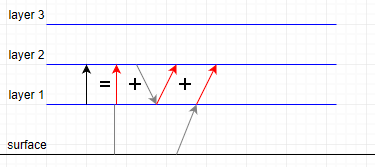
\includegraphics{scatter.PNG}
    \caption{Diagram showing how the expression of u1 (red arrow) was obtained.}
    \label{fig:scatter}
\end{figure}
in figure \ref{fig:scatter}, the black arrow represents shortwave radiation transmitted upward from layer 1 ($u_1$). It is the sum of three components indicated by red arrows (from left to right): a fraction of shortwave radiation reflected upward from the surface ($u_0$) which goes through layer 1 without any interaction ($u_0(1-s_1)$), a fraction of radiation transmitted downward from layer 2 ($d_2$) which scatters back as it reaches layer 1 ($0.5d_2s_1a_1$), and another fraction of radiation reflected upward from the surface ($u_0$) which scatters forward as it reaches layer 1 ($0.5u_0s_1a_1$). The 0.5 comes from the assumption of isotropic scattering.

\section*{Acknowledgement}
This project was started by Joel C. Schwartz as an off-line application. The Climate App was made available online by Anthony Courchesne. The current version is updated by Lan Xi Zhu. This project was supervised by Professor Nicolas Cowan from McGill University.


\newpage
\appendix
\section{Three-layer model without shortwave opacity}
The system of equations to solve are:
\begin{align*}
        T_0^4&=\frac{I(1-\alpha)}{\sigma}+\varepsilon_1  T_1^4 + \varepsilon_2  T_2^4(1-\varepsilon_1)+\varepsilon_3 T_3^4 (1-\varepsilon_2) (1-\varepsilon_1)\\
        &\\
        2 \varepsilon_1 T_1^4&=\varepsilon_1  T_0^4 + \varepsilon_1 \varepsilon_2  T_2^4 +\varepsilon_1 \varepsilon_3 T_3^4 (1-\varepsilon_2)\\
        &\\
        2\varepsilon_2  T_2^4&=\varepsilon_2  T_0^4 (1-\varepsilon_1) + \varepsilon_2 \varepsilon_1  T_1^4 + \varepsilon_2 \varepsilon_3  T_3^4\\
        &\\
        2 \varepsilon_3  T_3^4&=\varepsilon_3  T_0^4 (1-\varepsilon_1) (1-\varepsilon_2) + \varepsilon_3 \varepsilon_1  T_1^4(1-\varepsilon_2)+\varepsilon_3\varepsilon_2 T_2^4
\end{align*}
which is in fact identical to the system of equations used in the advanced model except for the shortwave absorption terms. The solutions are:

Surface:
\begin{equation*}
    T_0^4=\frac{2I(\alpha-1)(4-\varepsilon_1 \varepsilon_2 - \varepsilon_1 \varepsilon_3 - \varepsilon_2 \varepsilon_3 + \varepsilon_1 \varepsilon_2 \varepsilon_3)}{\sigma(\varepsilon_1-2)(\varepsilon_2-2)(\varepsilon_3-2)}
\end{equation*}

Layer 1:
\begin{equation*}
    T_1^4=\frac{I(\alpha-1)(4+2\varepsilon_2 -2\varepsilon_1 \varepsilon_2 + 2\varepsilon_3 - 2\varepsilon_1 \varepsilon_3 -3 \varepsilon_2 \varepsilon_3 + 2\varepsilon_1 \varepsilon_2 \varepsilon_3)}{\sigma(\varepsilon_1-2)(\varepsilon_2-2)(\varepsilon_3-2)}
\end{equation*}

Layer 2:
\begin{equation*}
    T_2^4=\frac{I(\alpha-1)(-2-\varepsilon_3+\varepsilon_2\varepsilon_3)}{\sigma(\varepsilon_2-2)(\varepsilon_3-2)}
\end{equation*}

Layer 3:
\begin{equation*}
    T_3^4 = \frac{I(\alpha-1)}{\sigma(\varepsilon_3-2)}.
\end{equation*}


\section{Shortwave absorption terms}\label{sec:short}
The solutions of the shortwave absorption terms, "$surf,l_1, l_2, l_3$", are:
\begin{align*}
    &surf=4I\cdot\frac{(a_3s_3 - 2s_3 + 2)[4A + 2a_1s_1(A - 1) +}{Aa_1^2a_2^2a_3s_1^2s_2^2s_3 - 4Aa_1^2a_2s_1^2s_2 -Aa_1^2a_3s_1^2s_3(a_2s_2 - 2s_2 + 2)^2 - }\\
    &\frac{a_2s_2(A - 1)(a_1s_1 - 2s_1 + 2) -}{4Aa_1a_2a_3s_1s_2s_3 + 16Aa_1s_1 - Aa_2^2a_3s_2^2s_3(a_1s_1 - 2s_1 + 2)^2 + 4Aa_2s_2(a_1s_1 - 2s_1 + 2)^2+}\\
    &\frac{4s_1(A - 1) - 2s_2(A - 1)(a_1s_1 - 2s_1 + 2) - 4]}{Aa_3s_3(a_1s_1 - 2s_1 + 2)^2(a_2s_2 - 2s_2 + 2)^2 - 2a_1a_2^2a_3s_1s_2^2s_3 + 8a_1a_2s_1s_2 +}\\
    &\frac{}{2a_1a_3s_1s_3(a_2s_2 - 2s_2 + 2)^2 + 8a_2a_3s_2s_3 - 32}\\
    &\\
    &l_1=4I\cdot\frac{s_1(a_3s_3 - 2s_3 + 2)[-Aa_1a_2s_1s_2(a_1 - 1) +}{Aa_1^2a_2^2a_3s_1^2s_2^2s_3 - 4Aa_1^2a_2s_1^2s_2 - Aa_1^2a_3s_1^2s_3(a_2s_2 - 2s_2 + 2)^2 -}\\
    &\frac{2Aa_1s_1s_2(a_1 - 1) + Aa_2s_2(a_1 - 1)(a_1s_1 - 2s_1 + 2) - }{4Aa_1a_2a_3s_1s_2s_3 + 16Aa_1s_1 - Aa_2^2a_3s_2^2s_3(a_1s_1 - 2s_1 + 2)^2 +}\\
    &\frac{4As_1(a_1 - 1) - 2As_2(a_1 - 1)(a_1s_1 - 2s_1 + 2) +}{4Aa_2s_2(a_1s_1 - 2s_1 + 2)^2 + Aa_3s_3(a_1s_1 - 2s_1 + 2)^2(a_2s_2 - 2s_2 + 2)^2 -  }\\
    &\frac{4A(a_1 - 1) + 4a_1 + 2a_2s_2(a_1 - 1) - 4s_2(a_1 - 1) - 4]}{2a_1a_2^2a_3s_1s_2^2s_3 +8a_1a_2s_1s_2 + 2a_1a_3s_1s_3(a_2s_2 - 2s_2 + 2)^2 + 8a_2a_3s_2s_3 - 32}\\
    &\\
    &l_2=4I\cdot\frac{s_2(a_3s_3 - 2s_3 + 2)[Aa_1^2s_1^2s_2(a_2 - 1) -}{Aa_1^2a_2^2a_3s_1^2s_2^2s_3 - 4Aa_1^2a_2s_1^2s_2 - Aa_1^2a_3s_1^2s_3(a_2s_2 - 2s_2 + 2)^2 -}\\
    &\frac{Aa_1^2s_1^2(a_2 - 1) + Aa_1s_1(a_2 - 1)(a_1s_1 - 2s_1 + 2) -}{4Aa_1a_2a_3s_1s_2s_3 + 16Aa_1s_1 - Aa_2^2a_3s_2^2s_3(a_1s_1 - 2s_1 + 2)^2 +}\\
    &\frac{2As_1(a_2 - 1)(a_1s_1 - 2s_1 + 2) - 4As_1(a_2 - 1) -}{4Aa_2s_2(a_1s_1 - 2s_1 + 2)^2 + Aa_3s_3(a_1s_1 - 2s_1 + 2)^2(a_2s_2 - 2s_2 + 2)^2 -}\\
    &\frac{As_2(a_2 - 1)(a_1s_1 - 2s_1 + 2)^2 + 4A(a_2 - 1) -}{2a_1a_2^2a_3s_1s_2^2s_3 + 8a_1a_2s_1s_2 +}\\
    &\frac{2a_1s_1s_2(a_2 - 1) + 2a_1s_1(a_2 - 1) + 4a_2 - 4]}{2a_1a_3s_1s_3(a_2s_2 - 2s_2 + 2)^2 + 8a_2a_3s_2s_3 - 32}\\
\end{align*}
\begin{align*}
    &l_3=I\cdot s_3\cdot\frac{(-a_3 + 1)[Aa_1^2a_2^2a_3s_1^2s_2^2s_3 - 4Aa_1^2a_2s_1^2s_2 -}{Aa_1^2a_2^2a_3s_1^2s_2^2s_3 -}\\
    &\frac{Aa_1^2a_3s_1^2s_3(a_2s_2 - 2s_2 + 2)^2 - 4Aa_1a_2a_3s_1s_2s_3 + 16Aa_1s_1 -}{ 4Aa_1^2a_2s_1^2s_2 -}\\
    &\frac{Aa_2^2a_3s_2^2s_3(a_1s_1 - 2s_1 + 2)^2 + 4Aa_2s_2(a_1s_1 - 2s_1 + 2)^2 +}{Aa_1^2a_3s_1^2s_3(a_2s_2 - 2s_2 + 2)^2 -}\\
    &\frac{Aa_3s_3(a_1s_1 - 2s_1 + 2)^2(a_2s_2 - 2s_2 + 2)^2 - 2a_1a_2^2a_3s_1s_2^2s_3 + 8a_1a_2s_1s_2 +}{4Aa_1a_2a_3s_1s_2s_3 + 16Aa_1s_1 -}\\
    &\frac{2a_1a_3s_1s_3(a_2s_2 - 2s_2 + 2)^2 + 8a_2a_3s_2s_3 - 32] + (a_3 - 1)(a_3s_3 - 2s_3 + 2)}{Aa_2^2a_3s_2^2s_3(a_1s_1 - 2s_1 + 2)^2 +}\\
    &\frac{[Aa_1^2a_2^2s_1^2s_2^2 - Aa_1^2a_2s_1^2s_2(a_2s_2 - 2s_2 + 2) - 2Aa_1^2a_2s_1^2s_2 +}{4Aa_2s_2(a_1s_1 - 2s_1 + 2)^2 +}\\
    &\frac{2Aa_1^2s_1^2s_2(a_2s_2 - 2s_2 + 2) + 4Aa_1^2s_1^2s_2 - 4Aa_1^2s_1^2 - 4Aa_1a_2s_1s_2 +}{Aa_3s_3(a_1s_1 - 2s_1 + 2)^2(a_2s_2 - 2s_2 + 2)^2 -}\\
    &\frac{4Aa_1s_1(a_1s_1 - 2s_1 + 2) + 8Aa_1s_1 - Aa_2^2s_2^2(a_1s_1 - 2s_1 + 2)^2 +}{ 2a_1a_2^2a_3s_1s_2^2s_3 + 8a_1a_2s_1s_2 +}\\
    &\frac{Aa_2s_2(a_1s_1 - 2s_1 + 2)^2(a_2s_2 - 2s_2 + 2) + 2Aa_2s_2(a_1s_1 - 2s_1 + 2)^2 - }{2a_1a_3s_1s_3(a_2s_2 - 2s_2 + 2)^2 +}\\
    &\frac{8As_1(a_1s_1 - 2s_1 + 2) -16As_1 - 2As_2(a_1s_1 - 2s_1 + 2)^2(a_2s_2 - 2s_2 + 2) - }{8a_2a_3s_2s_3 - 32}\\
    &\frac{4As_2(a_1s_1 - 2s_1 + 2)^2 +16A - 2a_1a_2^2s_1s_2^2 + 2a_1a_2s_1s_2(a_2s_2 - 2s_2 + 2) + 4a_1a_2s_1s_2 -}{}\\
    &\frac{4a_1s_1s_2(a_2s_2 - 2s_2 + 2) - 8a_1s_1s_2 + 8a_1s_1 + 8a_2s_2]}{}\\
\end{align*}



\end{document}